\chapter{Clustering}

\section{Support Vector Machines}
There are several libraries in R for using support vector machines (SVM).

\begin{itemize}
	\item kernlab
	\item e1071
\end{itemize}

Let's take a look at the kernlab library for now. To cluster data using an SVM with kernlab you need to pull out just the features you want and then convert that dataframe into a matrix. Then you can pass the resulting matrix into the ksvm function.

\begin{verbatim}
myData <- offABClustering[,c("logP", "phi31", "amp.I")]
myMatrix <- as.matrix(myData)
ksvmModel <- ksvm(myMatrix)
\end{verbatim}

The ksvm function will give you a model which you can then use to classify your data into the calculated clusters.

\begin{verbatim}
predictions <- predict(ksvmModel, myData)
offABClustering$cluster <- as.factor(predictions)
\end{verbatim}

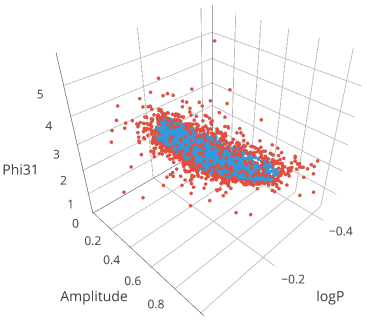
\includegraphics[]{images/ksvm_01.png}

\subsection{Kernels}
The ksvm function offers a few different kernels that you can use to change how it clusters the data. Each of these kernels will cluster the data into different ``shapes'' ranging from linear separations to rings. It looks like ksvm uses the ``rbfdot'' kernel by default.

\begin{itemize}
	\item rbfdot Radial Basis kernel "Gaussian"
	\item polydot Polynomial kernel
	\item vanilladot Linear kernel
	\item tanhdot Hyperbolic tangent kernel
	\item laplacedot Laplacian kernel
	\item besseldot Bessel kernel
	\item anovadot ANOVA RBF kernel
	\item splinedot Spline kernel
\end{itemize}

You can specify the kernel to be used in ksvm, by adding a kernel parameter where you pass in the name of the kernel you want to use as a string.

\begin{verbatim}
ksvmModel <- ksvm(myMatrix, kernel = "vanilladot")
\end{verbatim}

\begin{longtable}{ c c }
	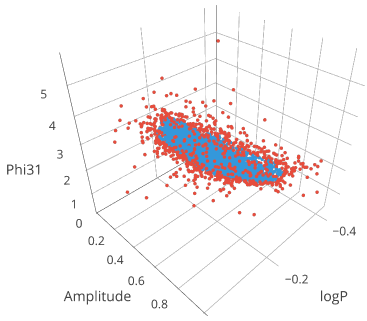
\includegraphics[width=0.3\paperwidth]{images/ksvm_rbfdot.png} & 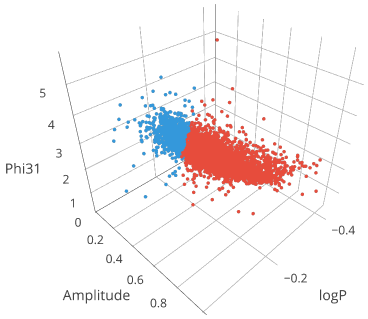
\includegraphics[width=0.3\paperwidth]{images/ksvm_polydot.png} \\
	rbfdot & polydot \\
	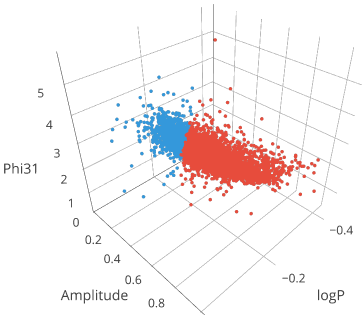
\includegraphics[width=0.3\paperwidth]{images/ksvm_vanilladot.png} & 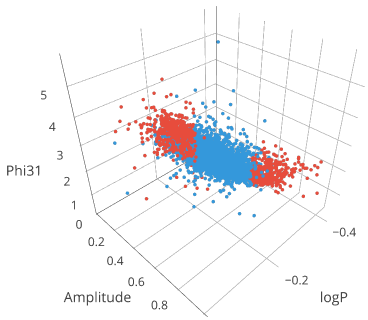
\includegraphics[width=0.3\paperwidth]{images/ksvm_tanhdot.png} \\
	vanilladot & tanhdot \\
	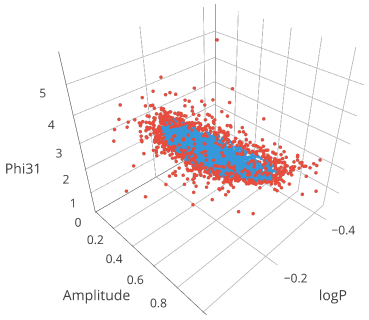
\includegraphics[width=0.3\paperwidth]{images/ksvm_laplacedot.png} & 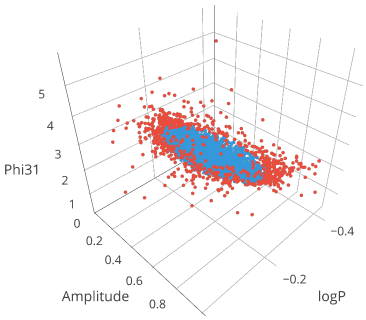
\includegraphics[width=0.3\paperwidth]{images/ksvm_besseldot.png} \\
	laplacedot & besseldot \\
	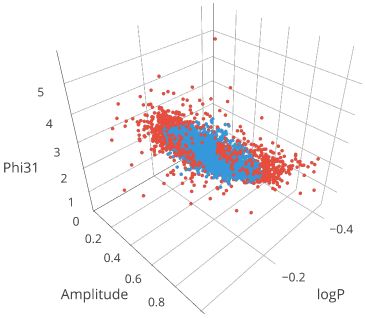
\includegraphics[width=0.3\paperwidth]{images/ksvm_anovadot.png} & 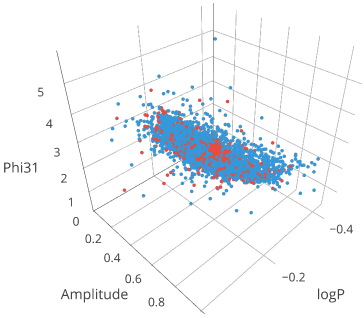
\includegraphics[width=0.3\paperwidth]{images/ksvm_splinedot.png} \\
	anovadot & splinedot \\
\end{longtable}

